\section{Stateful Firewall}


\subsection*{Kontext}


\subsection*{Problem}



\subsection*{Lösung}

\begin{figure}[H]
	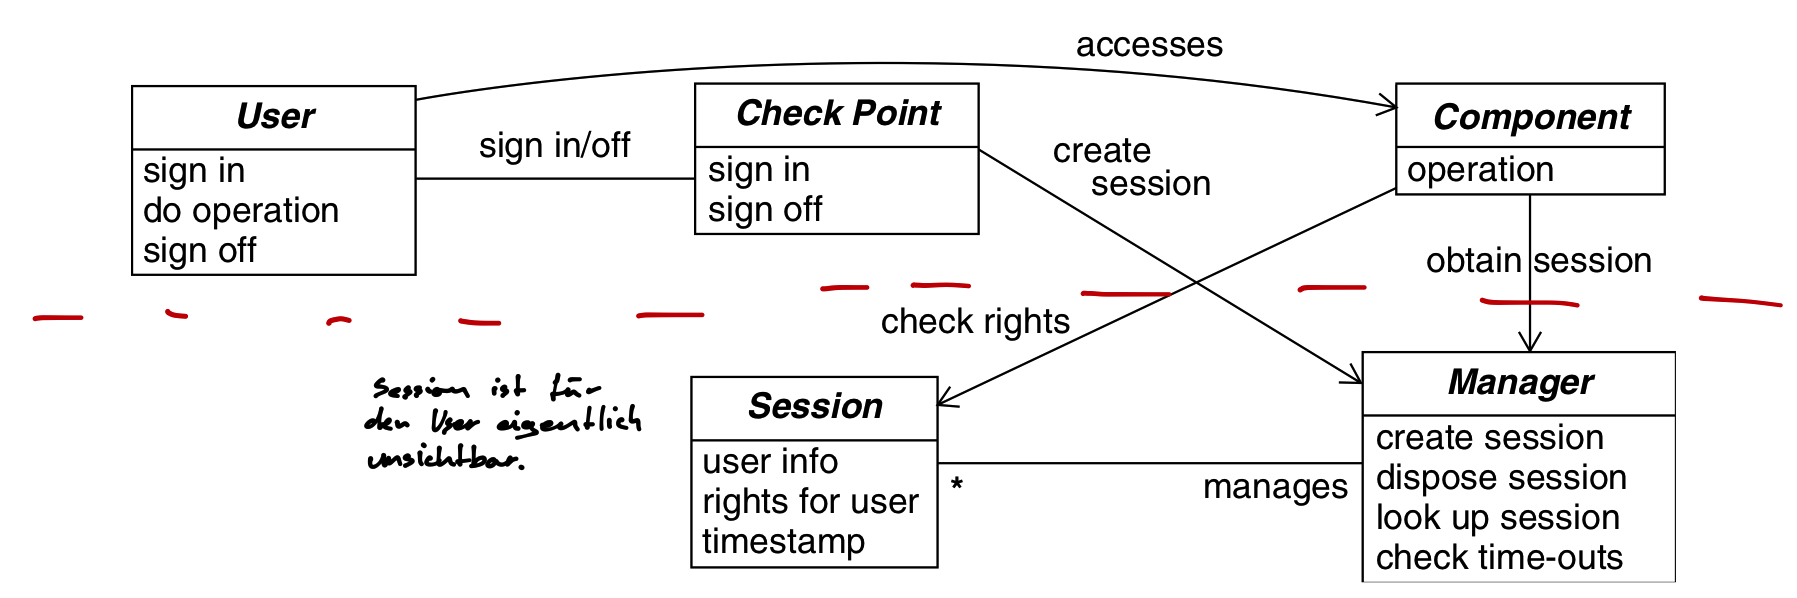
\includegraphics[width=\textwidth]{content/system-access-control-architecture/images/security-session-structure.png}
	\caption{Security Session: Schematischer Aufbau \cite{SecPatterns06}}
\end{figure}


\subsubsection*{Implementierung}
\begin{enumerate}
	\item 
\end{enumerate}

\subsection*{Vorteile}
\begin{itemize}
	\item 
\end{itemize}

\subsection*{Nachteile}
\begin{itemize}
	\item 
\end{itemize}

\subsection*{Reallife Beispiele}
\begin{itemize}
	\item 
\end{itemize}


\subsection*{Mögliche Prüfungsfragen}
\begin{itemize}
	\item 
\end{itemize}